\section{Results \& Discussion}

The training process for each model was evaluated using moving averages of the score, as illustrated in Fig. \ref{fig: Training curve - Infinite} and Fig. \ref{fig: Training curve - Finite}, because is it a clear indicator of convergence. The infinite situation converged after approximately '' iterations, which is a considerable amount less than for the finite situation, with '' iterations. This was a direct result of the difference in state spaces. 

The agent began around ~16 score in both situations because that is the middle of the possible values in the game. From here, q-values were updated based upon the agents moves, 
The two situations both converged at a  of  ~'', 

Stick values in the Q-table quickly converges to their value squared, as defined by equation \ref{reward}, the reward equation, which 

\begin{figure}[ht] 
    \centering
    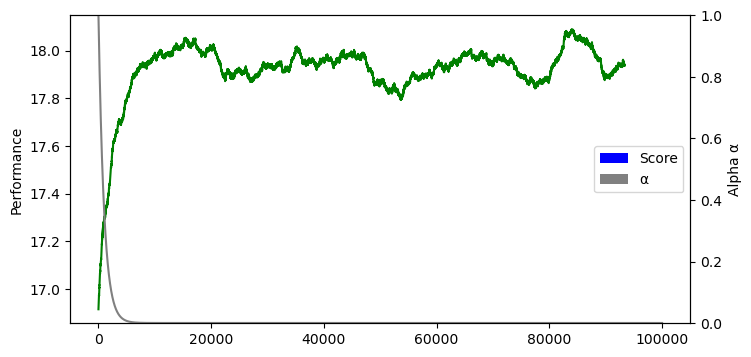
\includegraphics[width=\singlefigure]{figures/infinite_training_curve.png}
    \caption{Agent's training curve in the infinite situation.}
    \label{fig: Training curve - Infinite} 
\end{figure}

\begin{figure}[ht] 
    \centering
    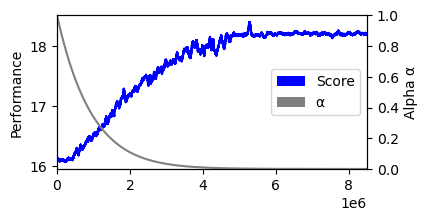
\includegraphics[width=\singlefigure]{figures/finite_training_curve.png}
    \caption{Agent's training curve in the finite situation.}
    \label{fig: Training curve - Finite} 
\end{figure}


Optimal hyperparameters were selected for each situation via a grid-search approach, in which a selection of hyperparameters were tested and compared. These hyperparameters are indicated in respective figures. 

The resulting optimal policies \(\pi^*\) are plotted in Fig. \ref{fig: Optimal policy - Infinite} for the infinite situation and Fig. \ref{fig: Optimal policy - Finite} for the finite situation. The infinite policy hits until 14 with no unused ace, and until 17 with an unused ace, which differs from the statistical stance of sticking on 17 irrespective of the held cards. The differences between this policy and the statistical optimum is due to the squared reward defined in \ref{eq: Score} and the absence of an active dealer. This drives the agent to be adverse to risk

\begin{figure}[ht]
    \centering
    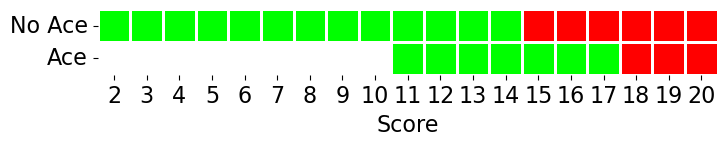
\includegraphics[width=\singlefigure]{figures/infinite_optimal_policy.png}
    \caption{Optimal policy for the infinite situation, with green indicating hit, and red indicating stick.}
    \label{fig: Optimal policy - Infinite} 
\end{figure}

The finite policy, in contrast, did not fully converge due to some states being very rarely entered, such as a 30\% chance of losing with a current score of 20. Despite this, 



\begin{figure}[ht]
    \centering
    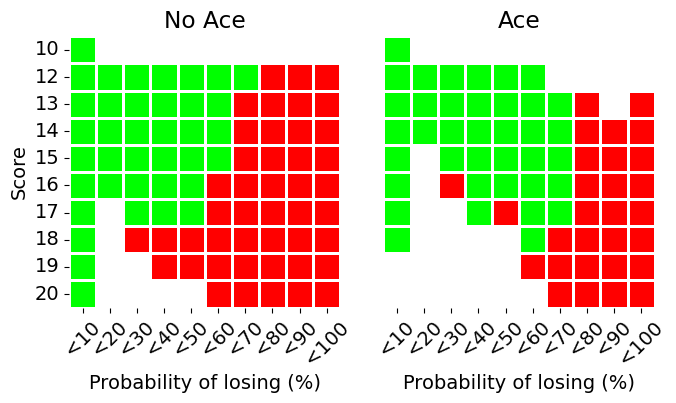
\includegraphics[width=\singlefigure]{figures/finite_optimal_policy.png}
    \caption{Optimal policy for the finite situation, with green indicating hit, and red indicating stick. Probability bins of 10\% increments are indicated accordingly. Missing policy points did not converge during training.}
    \label{fig: Optimal policy - Finite} 
\end{figure}

%To combat this issue, the rarely entered states could have been artificially entered, as this would have converged q-values irrespective of the agent's environment. 